\section{Theoretische Grundlagen}


\subsection{Radioaktivität}
\subsubsection{$\alpha$-Zerfall}

Zerfällt ein sogenannter Mutterkern $_Z^AX$ in einen Tochterkern $_{Z-2}^{A-4}Y$ und ein $He^{2+}$-Ion so spricht man von $\alpha$-Zerfall. Das $He^{2+}$-Teilchen wird $\alpha$-Teilchen genannt. Die Emission von $\alpha$-Teilchen ist ein quantenmechanischer Prozess, der durch Tunneln des $\alpha$-Teilchens durch die Potentialbarriere des Coulombpotentials des Kerns ermöglicht wird. $\alpha$-Teilchen zeigen ein diskretes Spektrum. Der $\alpha$-Zerfall ist für den Versuch nicht von Relevanz.

\subsubsection{$\beta$-Zerfall}

Man unterscheidet beim $\beta$-Zerfall zwischen $\beta^+$- und $\beta^-$-Zerfall und dem Elektroneneinfang.

\begin{figure}[H]
	\begin{minipage}{0.5\textwidth}
	\centering 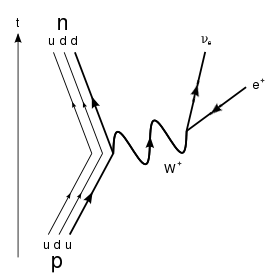
\includegraphics[width=\textwidth]{BilderTheorie/betaplus.png}
	\caption{$\beta^+$-Zerfall [en.wikipedia.org]}
	\end{minipage}
	\begin{minipage}{0.5\textwidth}
	\centering 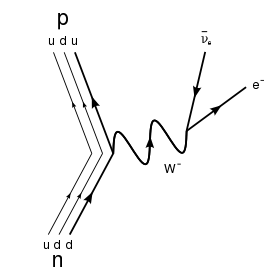
\includegraphics[width=\textwidth]{BilderTheorie/betaminus.png}
	\caption{$\beta^-$-Zerfall  [en.wikipedia.org]}	
	\end{minipage}
\end{figure}

Der $\beta^+$-Zerfall ist die Umwandlung eines Protons in ein Neutron mit Emission eines Positrons und eines Elektronenneutrinos:

$$ \beta^+: p^+ \rightarrow n^0 + e^+ + \nu_e $$

Dieser Zerfall ist wichtig für den Versuch, da auf diese Art Positronen erzeugt werden können, die mit Elektronen einen gebundenen Zustand eingehen können, nämlich das Positronium, welches in \ref{1} näher behandelt wird.
Der $\beta^-$-Zerfall ist die Umwandlung eines Neutrons in ein Proton, unter Emission eines Elektrons und eines Elektronen-Antineutrinos:

$$ \beta^-: n^0 \rightarrow p^+ + e^- + \bar \nu_e $$

Der $\beta^+$-Zerfall ist nur möglich für Protonen in einem Kern, da durch die Bindungsenergie die für den Prozess nötige Energie aufgebracht werden kann. Freie Protonen sind stabil.

Als weitere Art des $\beta$-Zerfall zählt man noch den Elektroneneinfang (EC, \emph{electron capture)}. Dieser kann stattfinden, wenn ein Elektron der untersten Schale (K-Schale), wegen dessen Aufenthaltswahrscheinlichkeit im Kern, vom Kern eingefangen wird und mit einem Proton zu einem Neutron reagiert. Dabei wird ein Elektronenneutrino emittiert:

$$ EC: p^+ + e^- \rightarrow n^0 + \nu_e $$

Der Elektroneneinfang gewinnt mit größeren Kernzahlen an Bedeutung, da dann die Aufenthaltswahrscheinlichkeit im Kern immer größer wird.

\subsubsection{$\gamma$-Zerfall}

Beim $\alpha$- und $\beta$-Zerfall gehen die Mutterkerne mit bestimmten Wahrscheinlichkeiten in verschiedene Anregungszustände der Tochterkerne über. Letztere zerfallen innerhalb einer sehr kurzen Zeit ($\sim 10^{-9}$ bis $10^{-12} s$) in den Grundzustand und emittieren dabei ein Photon mit Energien über 120 keV genannt $\gamma$-Quanten. Dieses $\gamma$-Quant wird entweder direkt vom Kern emittiert oder kann durch innere Konversion oder den Auger-Effekt seine Energie an Elektronen abgeben.

\subsection{Wechselwirkung von Photonen mit Materie \label{2}}

\subsubsection{Das Absorptionsgesetz}

Ein Photonenstrahl der einfallenden Intensität $I_0$ nimmt exponentiell mit der Dicke x einer durchquerten Materieschicht an Intensität ab. Es gilt also:

$$ I = I_0\cdot e^{-\mu x} $$

wobei $\mu$ der mediumabhängige (und photonenenergieabhängige) Absorptionkoeffizient ist. $\mu$ lässt sich als Summe der Absorptionskoeffizienten aller möglichen Wechselwirkungen von Photonen mit Materie schreiben, nämlich des Photoeffekts, des Compton-Effekts und der Paarbildung.

$$\mu = \mu_{Ph.} + \mu_{C} + \mu_{PB} $$

\subsubsection{Der Photoeffekt}

\begin{figure}[H]
	\begin{minipage}{0.59\textwidth}
	\centering 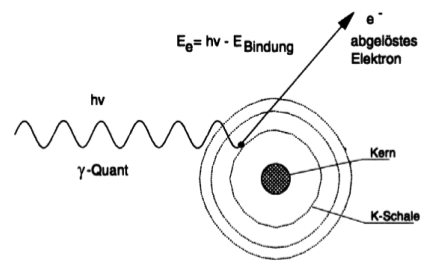
\includegraphics[width=\textwidth]{BilderTheorie/Photoeffekt.png}
	\caption{Photoeffekt}
	\end{minipage}
	\begin{minipage}{0.4\textwidth}
	Wenn ein $\gamma$-Quant ein Elektron aus der Atomhülle herausschlägt, spricht man vom Photoeffekt. Dieser Effekt tritt nur an gebundenen Elek\-tro\-nen auf. Die Energie des Photons geht zum größten Teil auf das Elektron, ein Teil wird jedoch als Rückstoßenergie vom Atom aufgenommen. Die Ab\-sorp\-tions\-wahrscheinlichkeit ist am größten in der K-Schale, also näher beim Kern. Der Photoeffekt dominiert gegenüber den anderen Effekten vor allem bei großen Atomen und Energien unter 100keV des Photons. Die entstandene Lücke wird dann durch ein weniger stark gebundenes oder freies Elektron aufgefüllt, wobei die Differenz der Bindungsenergien als Photon emittiert wird.
	\end{minipage}
\end{figure}

\subsubsection{Der Compton-Effekt}

\begin{figure}[H]
	\begin{minipage}{0.4\textwidth}
	Trifft ein Photon auf ein leicht gebundenes oder freies Elektron, so wird das Photon nicht ganz absorbiert, sondern gibt einen Teil seiner Energie an das Elektron ab und wird selbst gestreut. Durch die Streuung verliert das Photon somit an Energie, d.h. die Frequenz des gestreuten Quants ist kleiner. Der Compton-Effekt dominiert bei Energien zwischen 100 keV und einigen MeV.
	\end{minipage}
	\begin{minipage}{0.59\textwidth}
	\centering 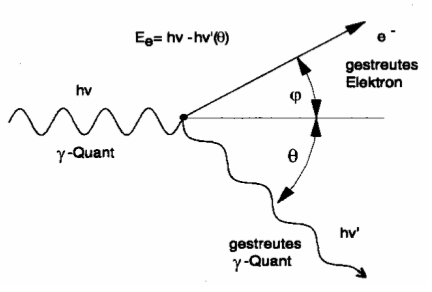
\includegraphics[width=\textwidth]{BilderTheorie/Comptoneffekt.png}
	\caption{Comptoneffekt}
	\end{minipage}

\end{figure}

\subsubsection{Die Paarbildung}

\begin{figure}[H]
	\begin{minipage}{0.5\textwidth}
	\centering 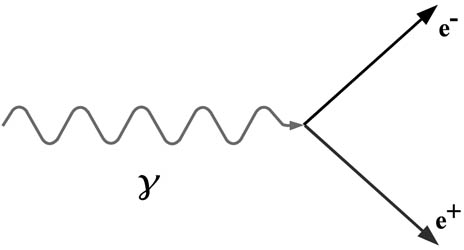
\includegraphics[width=\textwidth]{BilderTheorie/Paarbildung.jpg}
	\caption{Paarbildung}
	\end{minipage}
	\begin{minipage}{0.5\textwidth}
	Hat der $\gamma$-Quant mindestens die doppelte Ruheenergie eines Elektrons, also 1.022 MeV, so kann dieses im Feld eines Atomkerns (Stoßpartner für die Energie-Impuls-Erhaltung) ein Elektron-Positron-Paar erzeugen. 
	\end{minipage}
\end{figure}


\subsection{Szintillationszähler}

\begin{figure}[H]
	\centering 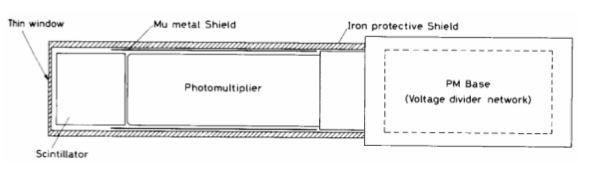
\includegraphics[width=\textwidth]{BilderTheorie/Szinti.png}
	\caption{Schema eines Szintillationszählers}
\end{figure}

Ein Szintillationszähler benutzt die in \ref{2} erklärten Ionisierungs-Phänomene um Photonen anhand geladener Strahlung nachzuweisen. Die geladene Strahlung löst Lichtblitze aus, die an einer Photokathode im Szintillator Elektronen freisetzen (Photoeffekt). Diese werden wiederum durch einen Photomultiplier verstärkt, so dass sie ein Signal mit einer messbaren Amplitude herausgeben, die der Energie des eingefallenen Quants proportional ist. Man unterscheidet zwischen organischen und anorganischen Szintillatoren. Bei dem organischen werden einzelne Moleküle angeregt, welche messbare Quanten emittieren. Beim anorganischen entstehen diese in einem Kristallgitter. Im Versuch benutzen wir anorganische NaI-Szintillationszähler.

\begin{figure}[H]
	\begin{minipage}{0.45\textwidth}
	Das Bändermodell erlaubt eine einfache Beschreibung des Verhaltens. Nämlich befinden sich bei tiefen Temperaturen alle Elektronen des Kristalls im sogenannten Valenzband. Absorbieren diese Elektronen energiereiche Strahlung, z.B. durch $\gamma$-Quanten (v.a. Photoeffekt), so werden diese angeregt und steigen auf höhere Energieniveaus. Reicht die Energie aus, so werden die Elektronen ins Leitungsband gehoben. Falls sie nicht groß genug ist um das Elektron vom Valenzband ins Leitungsband zu heben, so können sogenannte Exzitonen entstehen, lose gekoppelte Elektron-Loch-Paare (siehe Abb \ref{baendermodellszinti}). Die Exzitonen, können sich genau so wie die Leitungsband-Elektronen frei im Kristall bewegen und können unter Emission eines Photons wieder in den Grundzustand zurückkehren. 
	\end{minipage}
	\begin{minipage}{0.54\textwidth}
	\centering 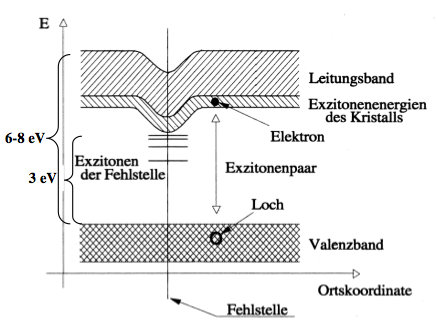
\includegraphics[width=\textwidth]{BilderTheorie/Bandmodell.png}
	\caption{Bändermodell beim NaI:Tl$^+$}
	\label{baendermodellszinti}
	\end{minipage}
\end{figure}
Eintreffende $\gamma$-Quanten haben Energien im Bereich von 0.1 bis 1 MeV, regen also mehrere hundert Elektronen gleichzeitig an. Wenn diese Elektron-Loch-Paare rekombinieren, entstehen neue Photonen, welche in den Photomultiplier geraten und dort verstärkt werden. Die Dotierung verformt lokal das Leitungsband und da diese Photonen vor allem an den Tl-Störstellen rekombinieren, reicht ihre Energie nicht aus um andere Elektronen ins Leitungsband anzuregen, somit können die Photonen nicht wieder vom Kristall absorbiert werden.


\subsection{Das Positronium \label{1}}
\subsubsection{Erzeugung}
\subsubsection{Ortho- und Parapositronium}
\subsubsection{Vernichtung}%und Auswahlregeln
\subsubsection{Energieniveaus}

\subsection{Der Zeeman-Effekt}

\subsection{Das Quenching}
\subsubsection{Quantenmechanische Störungstheorie}
\subsubsection{Quenching beim Positronium}

\subsection{Signalverarbeitung}